\chapter{Defining the problem}

\section{Iris flowers}
We are given sepal length, sepal width, petal length, petal width and our goal is to classify whether an iris flower is any of the following:

\begin{enumerate}
    \item Iris Setosa, see figure \ref{fig:setosa}. The image was taken from the Wikipedia article for Iris setosa~\cite{setosa}.
    \item Iris Versicolour, see figure \ref{fig:versicolour}. The image was taken from the Wikipedia article for Iris versicolour ~\cite{versicolor}.
    \item Iris Virginica, see figure \ref{fig:virginica}. The image was taken from the Wikipedia article for Iris Virginica ~\cite{virginica}.
\end{enumerate}
\begin{figure}
    \centering
    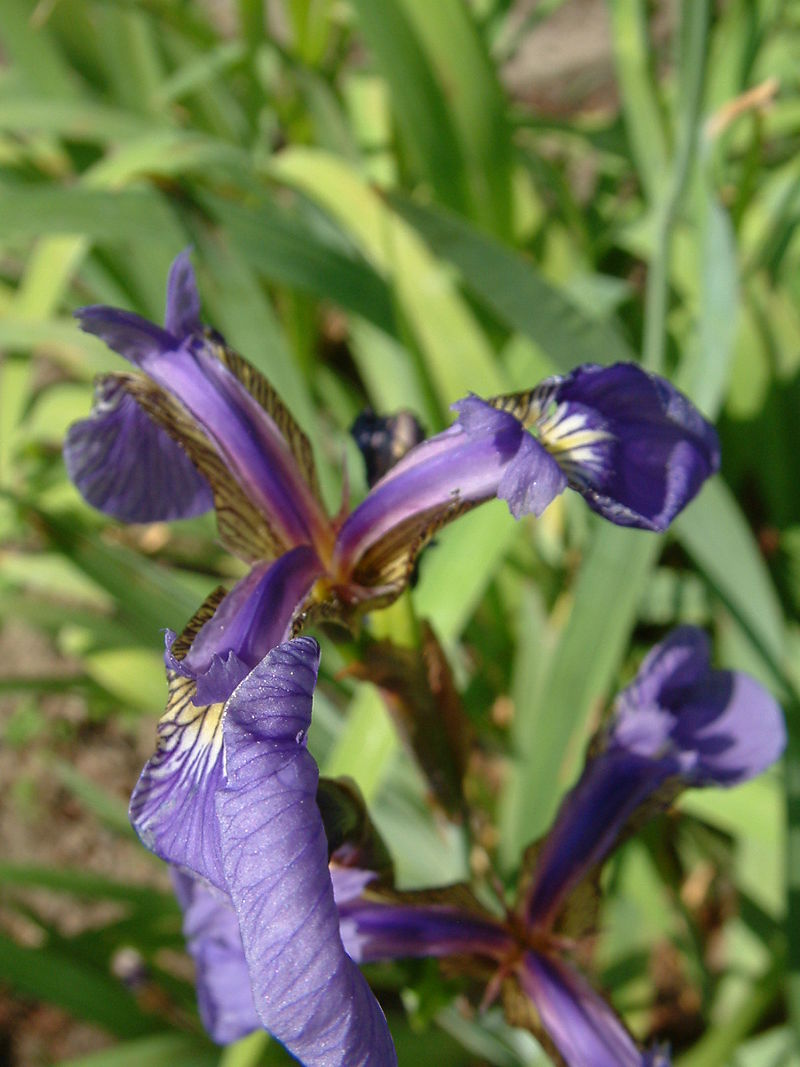
\includegraphics[scale=0.2]{setosa}
    \caption{Iris Setosa}
    \label{fig:setosa}
\end{figure}
\begin{figure}
    \centering
    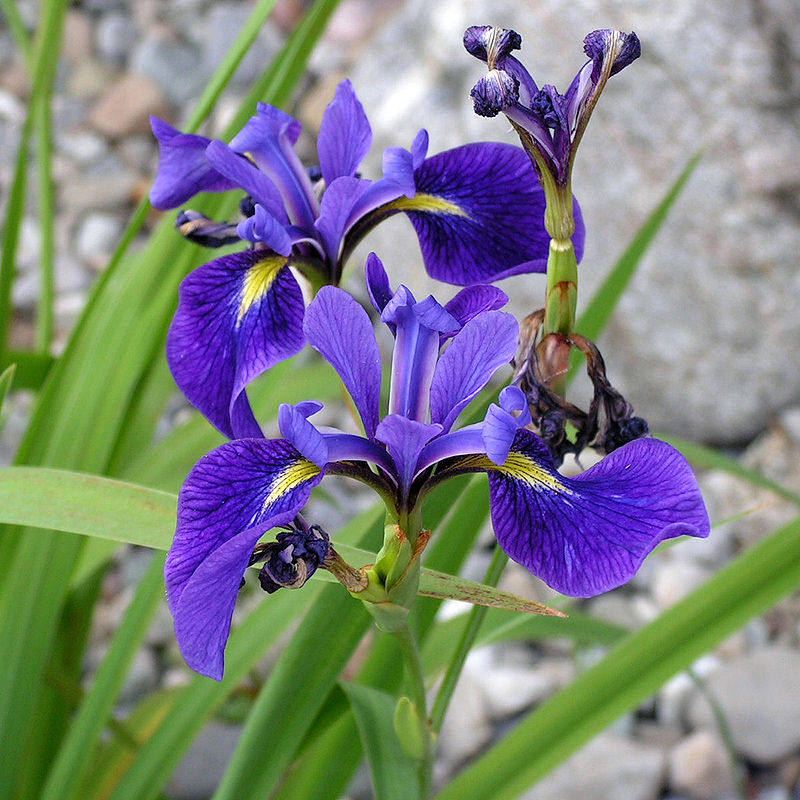
\includegraphics[scale=0.2]{versicolour}
    \caption{Iris Versicolour}
    \label{fig:versicolour}
\end{figure}
\begin{figure}
    \centering
    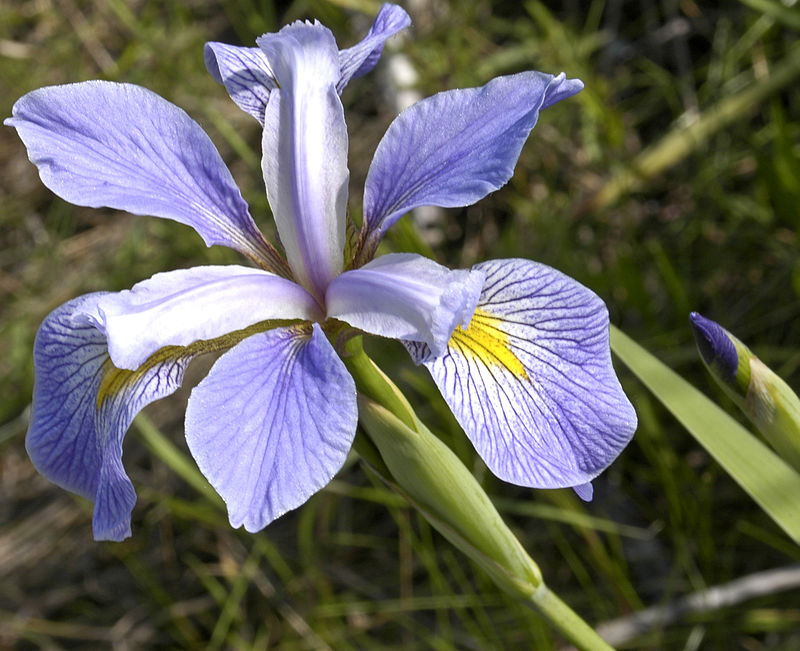
\includegraphics{virginica}
    \caption{Iris Virginica}
    \label{fig:virginica}
\end{figure}

\section{History of the dataset}
The dataset was introduced by Ronald Fischer in 1936 in his paper "The use of multiple measurements in taxonomic problems" ~\cite{setosa}. It is currently the most popular dataset in the UCI Machine Learning repository ~\cite{uci}
\section{Attribute information}
The dataset contains the following attributes ~\cite{iris}:
\begin{enumerate}
    \item Sepal length in cm
    \item Sepal width in cm 
    \item Petal length in cm 
    \item Petal width in cm
    \item Class - one of Iris Setosa, Iris Versicolour, Iris Virginica
\end{enumerate}
\section{First look at the dataset}